\chapter{神经系统神经退行性疾病的遗传机制} \label{chap:chap63}

神经系统的主要退行性疾病包括阿尔茨海默病、帕金森病以及三联体重复疾病(亨廷顿病和脊髓小脑性共济失调)。
这些疾病在美国影响超过600万人,在全球影响超过 2千5百万人。
尽管患者数量相对较少,但这些疾病给受影响者及其家人和朋友带来了不成比例的痛苦和经济困难。


大多数这些疾病会在中年或更晚的时候发作。
衰老本身可能会导致易感性。
最先出现的症状通常涉及精细运动控制的丧失。
亨廷顿病首先会表现为认知缺陷,阿尔茨海默病情况也是如此。
然而,最终结果是一样的:一段缓慢恶化的时期(通常为 10 到 20 年)剥夺了受折磨的患者的能力,并最终剥夺了他们的生命。


迟发性神经退行性疾病可分为两类:遗传性和散发性(即病因不明)。
阿尔茨海默病和帕金森病主要是散发性的;
尽管如此,仅影响少数患者的遗传形式为这些疾病的病理生理学提供了一些见解。
亨廷顿舞蹈病、脊髓小脑性共济失调、红梅突齿肌萎缩症和脊髓延髓肌萎缩症是遗传性的,是多聚谷氨酰胺或\textit{胞嘧啶-腺嘌呤-鸟嘌呤}三联体重复疾病的结果。


三联体重复疾病因由“动态”突变引起而引人注目:疾病蛋白质包含编码谷氨酰胺的\textit{胞嘧啶-腺嘌呤-鸟嘌呤}重复序列,并且可以在\textit{脱氧核糖核酸}复制过程中进行扩展。
不幸的是,\textit{胞嘧啶-腺嘌呤-鸟嘌呤}束越长,它越有可能进一步扩张,这就解释了预期的显著现象:
一个家庭中的年轻一代比他们的父母具有更长的重复序列,并且比他们的父母更早地出现更严重的症状。
鉴定这些疾病的分子基础识别有助于诊断并为最终治疗提供希望。



\section{亨廷顿病涉及纹状体的退化}

亨廷顿病通常在成年早期或中期发作,每 10 万人中有 5 到 10 人受到影响。
症状包括运动控制丧失、认知障碍和情感障碍。
运动问题最初最长表现为舞蹈症(不自主的、不规则的运动,起初涉及小关节,但随后逐渐影响腿部和躯干,使行走困难)。
快速、流畅的运动被僵硬和运动迟缓(异常缓慢的运动)所取代。


认知障碍(尤其是难以规划和执行复杂的功能)甚至可以在运动功能障碍之前通过正式的神经心理学测试来检测。
受影响的个体也可能有睡眠障碍和情感障碍,如抑郁、易怒和社交退缩。
大约 10\% 的患者会出现轻躁狂(精力增加),而一小部分患者会出现明显的精神病。


在成年患者中,疾病在发病后约 17 至 20 年不可避免地发展至死亡。
青少年发病的患者病程更快,通常仅在几年内就会出现运动迟缓、肌张力障碍(颈部、肩部和躯干痉挛)、僵硬(对肢体被动运动的抵抗)、癫痫发作和严重痴呆。


亨廷顿病的病理学标志是纹状体退化,它可以在症状出现前 10 年在神经影像学中表现出来。
尾状核比壳核受影响更大。
中棘神经元(纹状体中的一类抑制性中间神经元)的缺失会减少外部苍白球中神经元的抑制(第~\ref{chap:chap38}~章)。
由此产生的苍白球神经元过度活动抑制了丘脑底核,这可能是舞蹈样运动的原因。
随着疾病的进展和投射到内部苍白球的纹状体神经元退化,僵硬取代了舞蹈病。
皮层纹状体投射的破坏导致皮层变薄。
除了这种中枢神经系统病变外,患者还可能患有免疫系统和代谢紊乱、睾丸萎缩、心力衰竭、骨质疏松症和骨骼肌萎缩。
青少年亨廷顿病病例更严重,病理进展更迅速、范围更广;
例如,可能发生小脑浦肯野细胞退化。


亨廷顿病是一种常染色体显性遗传病,也是最早使用多态\textit{脱氧核糖核酸}标记绘制基因图谱的人类疾病之一。
它是由翻译的\textit{胞嘧啶-腺嘌呤-鸟嘌呤}重复序列的扩展引起的,该重复序列编码亨廷顿蛋白中的谷氨酰胺束。
正常或野生型等位基因有 6 到 34 个重复,而致病等位基因通常有 36 个或更多重复,当从一代传递到下一代时,尤其是通过父系生殖细胞传递时,这些等位基因非常不稳定。
疾病严重程度、发病年龄和进展速度与重复长度相关;
重复次数为 36 至 39 次的个体发病较晚且病情较轻,而重复次数超过 40 次的个体发病较早且病程较重。
那些携带超过 75 个重复的人将在幼年时患上这种疾病。


扩大的谷氨酰胺束导致亨廷顿蛋白的功能增加,这是一种在自然界中从无脊椎动物到哺乳动物都保存得很好的348-kDa蛋白。
它以可溶性细胞质蛋白的形式在整个大脑中表达,一小部分存在于细胞核中。
它在体树突区域和轴突中特别丰富,并且已被发现与微管相关。
尽管其确切功能尚不完全清楚,但亨廷顿蛋白对于正常的胚胎发育是必不可少的。
基于在新陈代谢、蛋白质周转、货物运输和基因表达中起作用的多种蛋白质相互作用物,假设亨廷顿蛋白起分子支架的作用。
它的大尺寸、稳定性和在多种构象之间转换的能力表明它可以将多种蛋白质聚集在一起形成大分子复合物。


亨廷顿有多个蛋白质结构域,其中研究得最好的是 N 末端区域,它包含聚谷氨酰胺扩展和核定位信号。
N 末端区域由一个两亲性 $\alpha$ 螺旋组成,它创造了一个对蛋白质在内质网中的保留至关重要的结构。
N 末端通过乙酰化、泛素化、磷酸化和苏木化进行广泛的翻译后修饰,所有这些都会影响亨廷顿清除和亚细胞定位。
有趣的是,外显子 1 中的多聚谷氨酰胺重复序列后面是一个富含脯氨酸的结构域,与其他外显子不同,该结构域在进化过程中保守性很差。


N 末端外的其余 66 个外显子(约占蛋白质的 98\%)的表征远没有那么好。
几个 HEAT 重复序列对于蛋白质-蛋白质相互作用很重要。
这些相互作用允许亨廷顿蛋白采用大量三维构象(体外多达 100 个)。
此外,HTT 基因产生两种不同的\textit{信使核糖核酸}转录物,一种是短的,一种是长的。
长形式包含一个额外的 3' 非翻译区域,并在大脑中丰富。
罕见的可变剪接产生跳过外显子 10、12、29 和 46 或包括外显子 41b 或内含子 28 片段的亚型,但它们的重要性尚未确定。
这些亚型的多样性在发育过程中可能很重要,并且可以扩大亨廷顿蛋白可用的蛋白质相互作用的多样性。



\section{脊髓延髓肌萎缩是由雄激素受体功能障碍引起的}

\textit{脊延髓肌萎缩症}是本章讨论的神经退行性疾病中唯一的 X 连锁疾病。
它是由雄激素受体蛋白中翻译的\textit{胞嘧啶-腺嘌呤-鸟嘌呤}重复序列的扩展引起的,雄激素受体蛋白是类固醇激素受体家族的一员。
只有雄性表现出症状:
突变的雄激素受体只有定位于细胞核时才具有毒性,并且这种定位依赖于激素雄激素。


近端肌肉无力通常是主要症状;
最终,远端和面部肌肉也会变弱。
肌肉萎缩很明显,继发于运动神经元的退化。
雄激素功能的丧失通常会导致男性乳房发育症(男性乳房组织的生长)、晚期性腺机能减退和不育。
因为因其他原因失去雄激素受体功能的个体不会发生运动神经元变性,似乎\textit{脊延髓肌萎缩症}中的谷氨酰胺扩张会导致导致第二性征的部分功能丧失和损害神经元并产生的部分功能获得神经功能障碍。



\section{遗传性脊髓小脑性共济失调症状相似,但病因不同}

\textit{脊髓小脑共济失调}和\textit{齿状核红核苍白球路易体萎缩症}的特征是小脑、脊髓束和各种脑干核团的功能障碍。
基底神经节、大脑皮层和周围神经系统也会受到影响(表~\ref{tab:63_1})。


\begin{table}[htbp]
	\caption{不稳定\textit{胞嘧啶-腺嘌呤-鸟嘌呤}三核苷酸重复序列引起神经退行性疾病的遗传模式及主要临床特征} \label{tab:63_1} \centering
	\begin{tabular}{llll}
		\toprule
		疾病 & 遗传 & 典型表现特征 & 受影响的主要区域\\
		\midrule
		\textit{脊延髓肌萎缩症} & X连锁隐性 & \makecell{肌肉痉挛、虚弱、女性\\乳房发育不良} & 下运动神经元和前角细胞 \\
		\textit{亨廷顿病} & 常染色体显性 & \makecell{认知障碍、舞蹈病、抑郁\\、易怒} & 纹状体、皮层 \\
		\textit{类亨廷顿病2型} & 常染色体显性 & \makecell{认知障碍、舞蹈病、抑郁\\、易怒} & 纹状体、皮层 \\
		\textit{脊髓小脑共济失调1型} & 常染色体显性 & \makecell{\textit{眼跳}、共济失调、构音\\障碍、平衡、眼球震颤} & 浦肯野细胞、脑干 \\
		\textit{脊髓小脑共济失调2型} & 常染色体显性 & \makecell{共济失调、反射减退\\、缓慢\textit{眼跳}} & \makecell{浦肯野细胞、颗粒细胞、\\下橄榄} \\
		\textit{脊髓小脑共济失调3型} & 常染色体显性 & \makecell{共济失调、凝视引起\\的眼球震颤、眼睛肿胀、\\肌张力障碍、痉挛} & \makecell{脑桥神经元、黑质、\\前角细胞} \\
		\textit{脊髓小脑共济失调6型} & 常染色体显性 & \makecell{共济失调,迟发\\(大于50岁)} & 浦肯野细胞、颗粒细胞 \\
		\textit{脊髓小脑共济失调7型} & 常染色体显性 & \makecell{共济失调、视网膜变性引\\起的视觉损失、听力损失} & \makecell{浦肯野细胞,视网膜\\(视锥杆变性)} \\
		\textit{脊髓小脑共济失调8型} & 常染色体显性 & 扫描性构音障碍、共济失调 & 浦肯野细胞 \\
		\textit{脊髓小脑共济失调10型} & 常染色体显性 & 共济失调和癫痫发作 & 浦肯野细胞 \\
		\textit{脊髓小脑共济失调12型} & 常染色体显性 & \makecell{早期手臂震颤、反射亢进\\、共济失调} & \makecell{浦肯野细胞、皮层\\和小脑萎缩} \\
		\textit{齿状核红核苍白球路易体萎缩症} & 常染色体显性 & 痴呆、共济失调、舞蹈病 & \makecell{齿状核、红核、苍白球、\\丘脑底核、小脑皮层、皮层} \\
		\bottomrule
	\end{tabular}
\end{table}


所有\textit{脊髓小脑共济失调}共有的两个临床特征,共济失调和构音障碍,是小脑功能障碍的迹象。
这些通常出现在成年中期并逐渐恶化,最终导致无法行走和无法理解语言。
晚期疾病的脑干功能障碍导致难以保持气道畅通;
患者常死于吸入性肺炎。
一些\textit{脊髓小脑共济失调}与其他症状相关,例如舞蹈病、视网膜病变或痴呆,但这些症状变化太大而无法支持鉴别诊断。
即使是同一家庭中的个体也可能呈现出截然不同的临床表现。
因此,虽然\textit{脊髓小脑共济失调}是单基因孟德尔疾病,但个体基因构成和环境影响会影响临床病理图。


例如,\textit{马查多-约瑟夫病}和\textit{脊髓小脑共济失调 3 型}在发现它们是由同一基因突变引起之前,在临床上一直被视为不同的疾病。
临床上的混乱是由历史事故引起的。
最先研究的亚速尔群岛后裔家庭最显著的特征是眼睛凸出、面部语言肌束震颤、帕金森症和肌张力障碍;
这种综合症被命名为\textit{马查多-约瑟夫病}。
随后,一组欧洲遗传学家研究了具有更容易让人联想到 \textit{脊髓小脑共济失调1型}症状的患者,除了典型的共济失调和构音障碍之外,还有超快的\textit{眼跳}和活跃的反射。
因此,这一症状群被称为\textit{脊髓小脑共济失调3型}。
这两种疾病的遗传位点相同花了几年时间才变得清晰,但仍然使用两个名称(\textit{马查多-约瑟夫病}和\textit{脊髓小脑共济失调3型})。
我们现在知道,在最初的两组患者中观察到的差异至少部分归因于\textit{胞嘧啶-腺嘌呤-鸟嘌呤}重复长度的差异。
尽管如此,由遗传变异引起的其他蛋白质活性的差异也可能在起作用。


如图~\ref{fig:63_1}~所示,每种共济失调的发病年龄取决于基因中\textit{胞嘧啶-腺嘌呤-鸟嘌呤}重复的数量,尽管不同重复长度的毒性取决于蛋白质背景。
例如,\textit{脊髓小脑共济失调6型}中的\textit{胞嘧啶-腺嘌呤-鸟嘌呤}扩展是所有\textit{脊髓小脑共济失调}中最短的:正常等位基因的重复少于 18 个,病理重复只有 21 到 33 个。
然而,在其他\textit{脊髓小脑济失调} 中,长度完全相同的束是完全非致病性的。
事实上,负责\textit{脊髓小脑共济失调7型}的基因通常可以容忍几十个\textit{胞嘧啶-腺嘌呤-鸟嘌呤}重复,并且在疾病状态下,可以扩展到数百个\textit{胞嘧啶-腺嘌呤-鸟嘌呤},这是任何\textit{脊髓小脑共济失调}中所见的最大扩展。



\begin{figure}[htbp]
	\centering
	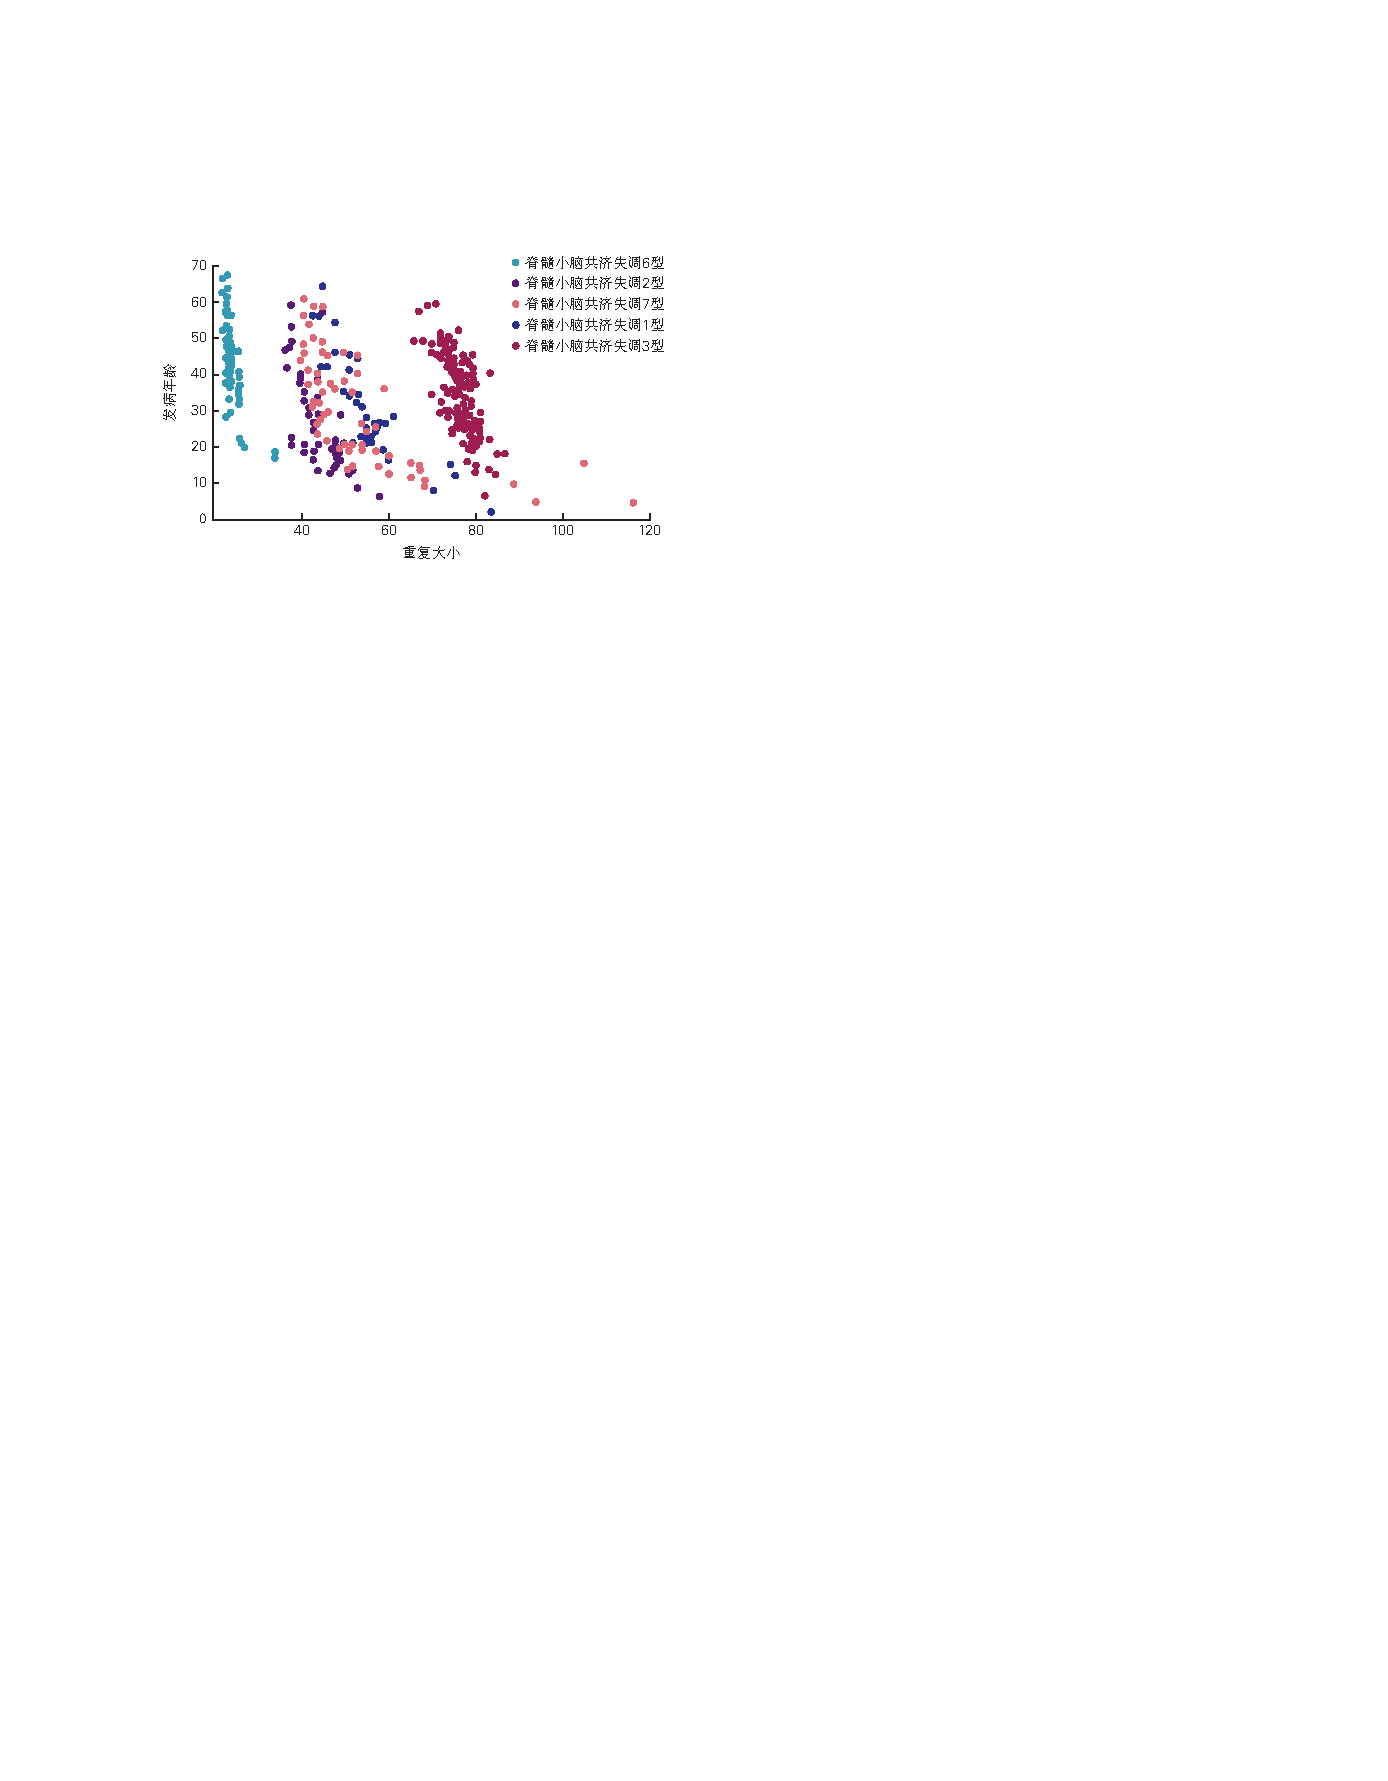
\includegraphics[width=0.7\linewidth]{chap63/fig_63_1}
	\caption{\textit{胞嘧啶-腺嘌呤-鸟嘌呤}重复序列的长度与\textit{脊髓小脑共济失调}的发病年龄呈负相关。
		\textit{胞嘧啶-腺嘌呤-鸟嘌呤}道越长,特定疾病的发作越早。
		然而,特定的重复长度会因宿主蛋白的不同而产生不同的结果。
		例如,\textit{胞嘧啶-腺嘌呤-鸟嘌呤}的 52 次重复导致 2 型脊髓小脑性共济失调(\textit{脊髓小脑共济失调2型})的青少年发病,1 型脊髓小脑性共济失调(\textit{脊髓小脑共济失调1型})的成人发病,以及 3 型脊髓小脑性共济失调(\textit{脊髓小脑共济失调3型})的无疾病。}
	\label{fig:63_1}
\end{figure}


除了容忍不同的\textit{胞嘧啶-腺嘌呤-鸟嘌呤}重复长度外,多聚谷氨酰胺疾病中突变基因的基因产物在功能上也有很大差异:


\textit{脊髓小脑共济失调1型}中的基因产物\textit{共济失调蛋白-1}主要是一种核蛋白,它与\textit{Capicua转录阻抑蛋白}形成复合物。
扩大的谷氨酰胺束改变了 ATXN1 与小脑中\textit{Capicua转录阻抑蛋白}的相互作用,这有助于解释该区域易受\textit{脊髓小脑共济失调1型}病理生理学影响的原因。


\textit{脊髓小脑共济失调2型}是由 ATXN2 中的\textit{胞嘧啶-腺嘌呤-鸟嘌呤}三核苷酸扩增引起的。
Atxn2 的遗传消融增加了全局转录本丰度,表明它可能作为\textit{核糖核酸}结合蛋白起作用。
最近的研究表明,它与 TDP43 相互作用,TDP43 是一种参与肌萎缩侧索硬化(ALS10)的蛋白质,ATXN2 的突变可能导致肌萎缩侧索硬化。


蛋白质清除受损是\textit{脊髓小脑共济失调}的一个主题,因为致病蛋白质水平升高似乎推动了发病机制。
在\textit{脊髓小脑共济失调3型}的情况下,这种关系更为直接,因为\textit{共济失调蛋白-3}是一种去泛素化酶,而扩展版本不能从准备清除的蛋白质中去除泛素。
最近,ATXN3 与\textit{脱氧核糖核酸}损伤修复有关。


\textit{脊髓小脑共济失调6型}中受影响的基因产物 CACNA1A 是电压门控 \ce{Ca^2+} 通道的 $\alpha$1A 亚基;
有趣的是,在患有发作性共济失调和家族性偏瘫性偏头痛的患者中,已经报道了该基因的功能丧失突变(不是由\textit{胞嘧啶-腺嘌呤-鸟嘌呤}重复引起的功能获得)。


在 \textit{脊髓小脑共济失调17型}中,受影响的基因产物是 TATA 盒结合蛋白,一种必需的转录因子。


Atrophin-1,\textit{齿状核红核苍白球路易体萎缩症}中的致病蛋白,根据其在果蝇中可能的直系同源物的功能研究,被认为是一种辅阻遏物。


尽管存在这些差异,一些致病机制可能与多聚谷氨酰胺疾病相同,本章后文将讨论这一点。


编码区中的\textit{胞嘧啶-腺嘌呤-鸟嘌呤}重复并不是\textit{脊髓小脑共济失调}中发生的唯一动态突变(表~\ref{fig:63_2})。
\textit{脊髓小脑共济失调8型}涉及在没有开放阅读框的转录\textit{核糖核酸}的 3' 非翻译区的相反链上扩展\textit{胞嘧啶-腺嘌呤-鸟嘌呤}束及其互补 CTG 重复序列。
导致\textit{脊髓小脑共济失调12型}的突变是\textit{胞嘧啶-腺嘌呤-鸟嘌呤}重复序列,但它发生在蛋白磷酸酶 2A 的脑特异性调节亚基上游 5' 的非编码区。
\textit{脊髓小脑共济失调10型}是由新基因内含子中五核苷酸(ATTCT)重复序列的大量扩增引起的。


\begin{figure}[htbp]
	\centering
	\includegraphics[width=0.97\linewidth]{chap63/fig_63_2}
	\caption{三核苷酸重复疾病和帕金森病中神经元变性的主要部位说明了神经元选择性。
		A. 最常受成人发病影响的大脑区域(见表~\ref{tab:63_1})。
		B. \textit{肌萎缩侧索硬化}和\textit{脊延髓肌萎缩症}的神经病理学比较。}
	\label{fig:63_2}
\end{figure}


到目前为止,总共确定了 33 种\textit{脊髓小脑共济失调}。
对于其潜在发病机制得到更好理解的\textit{脊髓小脑共济失调},最有希望的治疗方法似乎是降低疾病驱动蛋白的水平。
在\textit{脊髓小脑共济失调7型}小鼠模型中,通过\textit{核糖核酸}干扰减少突变型和野生型 ATXN7 的数量极大地改善了疾病的行为和病理体征。
同样,在\textit{脊髓小脑共济失调1型}的果蝇和小鼠模型中,RAS-\textit{有丝分裂原活化蛋白激酶}-MSK1 通路的几个组分的遗传或药理学下调会降低 ATXN1 水平并抑制神经变性。



\section{帕金森病是老年人常见的退行性疾病}

帕金森病是一种更常见的神经退行性疾病,影响了大约 3\% 的 65 岁以上人口。
帕金森病患者遭受静息性震颤、运动迟缓、僵硬以及发起和维持运动的能力受损。
受影响的人以一种独特的蹒跚步态行走,他们的平衡往往不稳定。
自发的面部运动大大减少,形成一种无表情的,面具般的外观。
帕金森病的病理特征是多巴胺能神经元的逐渐丧失,主要在黑质致密部(第~\ref{chap:chap38}~章),以及称为路易体和路易神经突的蛋白质聚集体在整个大脑中的积累。


虽然大多数帕金森病病例是散发性的,但对罕见的家族性病例(可以是常染色体显性遗传或隐性遗传)的研究提供了对这种疾病的病理生理学的深入了解,并揭示了疾病的新危险因素。
迄今为止,已经绘制了几个基因位点(指定为 PARK1–PARK22),并且除了四个这些位点(PARK3、PARK10、PARK12 和 PARK16)之外的所有基因都已被识别(表~\ref{tab:63_3})。
在这些映射的基因座中,研究最多和表征最多的是 PARK1/4、PARK2、PARK6 和 PARK7。
在这里,我们关注某些形式的帕金森病的遗传基础如何为散发性帕金森病的提供见解。


\begin{table}[htbp]
	\caption{遗传性帕金森病的遗传学及主要临床特征} \label{tab:63_3} \centering
	\begin{tabular}{lllll}
		\toprule
		疾病 & 发生地 & 遗传方式 & 基因 & 主要特征\\
		\midrule
		PARK1/4 & 4q21 & 常染色体显性 & SNCA & 早发、僵硬和认知障碍 \\
		PARK2 & 6q26 & 常染色体隐性 & PARKIN & 青少年发病和肌张力障碍 \\
		PARK3 & 2p13 & 常染色体显性 & 未知 & 成人发病,痴呆 \\
		PARK5 & 4p13 & 常染色体显性 & UCHL1 & 成人发病 \\
		PARK6 & 1p36.12 & 常染色体隐性 & \makecell[l]{蛋白酪氨酸\\磷酸酶基因\\诱导假定激酶1} & 早发性、肌张力障碍 \\
		PARK7 & 1p36.21 & 常染色体隐性 & DJ1 & 早发、行为障碍、肌张力障碍 \\
		PARK8 & 12q12 & 常染色体显性 & LRRK2 & 经典帕金森病 \\
		PARK9 & 1p36.13 & 常染色体隐性 & ATP13A2 & 青少年或早发,认知障碍 \\
		PARK10 & 1p32 & 常染色体显性 & 未知 & 经典帕金森病 \\
		PARK11 & 2q37.1 & 常染色体显性 & GIGYF2 & 成人发病,认知障碍 \\
		PARK12 & Xq21-25 & X连锁 & 未知 & 未知 \\
		PARK13 & 2p13.1 & 常染色体显性 & Omi/HtrA2 & 经典帕金森病 \\
		PARK14 & 22q13.1 & 常染色体隐性 & PLA2G6 & 早发、认知障碍、肌张力障碍。 \\
		PARK15 & 22q12.3 & 常染色体隐性 & FBXO7 & 青少年发病或早发 \\
		PARK16 & 1q32 & 未知 & 未知 & 未知 \\
		PARK17 & 16q11.2 & 未知 & VPS35 & 成人发病、认知障碍、肌张力障碍 \\
		PARK18 & 6p21.3 & 未知 & EIF4G1 & 经典帕金森病 \\
		PARK19a/b & 1p31.3 & 常染色体隐性 & DNAJC6 & 青少年或早发,认知障碍 \\
		PARK20 & 21q22.11 & 常染色体隐性 & SYNJ1 & 早发,癫痫发作 \\
		PARK21 & 3q22 & 常染色体显性 & DNAJC13 & 经典帕金森病 \\
		PARK22 & 7p11.2 & 常染色体显性 & CHCHD2 & 经典帕金森病 \\
		\bottomrule
	\end{tabular}
\end{table}


帕金森病 1/4 型(4q2-22)是由编码 $\alpha$-突触核蛋白的 SNCA 基因突变引起的显性遗传性帕金森病的基因座。
(与\textit{马查多-约瑟夫病}和\textit{脊髓小脑共济失调3型}一样,Park1 和 Park4 最初被认为是两个不同的变体。)SNCA 基因座中的变体与散发性帕金森病的风险增加有关,并且 SNCA 中的几个突变改变了膜的构象 $\alpha$-突触核蛋白的结合部分并使其聚集。
SNCA 的重复和三次重复也已被确定为常染色体显性帕金森病的原因,表明即使是野生型 $\alpha$-突触核蛋白水平升高也可能导致疾病。
SNCA 重复患者的病程类似于散发病例,但三次重复患者表现为发病较早、进展较快的疾病,具有痴呆和幻觉等非典型特征。


SNCA突变患者与散发性帕金森病患者不同,发病年龄较早(平均45岁),表现为震颤较少、强直、认知能力下降、肌阵挛、中枢性通气不足、体位性低血压和尿失禁。


常染色体隐性青少年帕金森病的特征是早发性肌张力障碍、活跃的深腱反射和小脑体征以及帕金森病的典型体征,所有这些都早在 3 岁时就出现了。
PARK2、PARK6 和 PARK7 中的突变分别编码帕金蛋白、\textit{蛋白酪氨酸磷酸酶基因诱导假定激酶1}和蛋白去糖酶 DJ-1,已被证实是这种疾病的原因。
PARK2 中的突变比 PARK6 和 PARK7 中的突变更频繁,并且已经确定了 60 多种不同的失活突变;
因此,常染色体隐性青少年帕金森病是由基因产物功能丧失而不是功能获得引起的。
病理学的特征还在于多巴胺能神经元的丢失,但路易体不像散发性或 PARK1/4 病例那样常见。
Parkin 是 RING 指家族的 E3 泛素连接酶,可将活化的泛素转移到蛋白质中的赖氨酸残基,这些残基将被蛋白酶体降解。
对\textit{黑腹果蝇}的研究表明,parkin 和\textit{蛋白酪氨酸磷酸酶基因诱导假定激酶1}共同促进健康的线粒体。
有趣的是,常染色体隐性青少年帕金森病的第三个原因 DJ-1 也参与线粒体功能,充当氧化应激传感器。


并非所有帕金森病的遗传原因都表现出完全外显率。
编码富含亮氨酸的重复激酶 2(LRRK2、PARK8)的基因突变就是这种情况。
有趣的是,LRRK2 突变是散发性帕金森病的危险因素。
帕金森病的另一个遗传风险因素是编码\textit{葡糖脑甘酯酶-1}的基因:
\textit{葡糖脑甘酯酶-1}突变的杂合子携带者在以后的生活中患帕金森病的风险增加,而纯合子携带者会患上一种称为戈谢病的隐性疾病。
毫无疑问,帕金森病还有其他遗传风险因素,并且我们正在努力识别它们。



\section{普遍表达的基因受损后发生选择性神经元丢失}

这些神经退行性疾病的一个令人费解的方面是,改变的基因产物不仅在神经系统广泛而大量地表达,而且在其他组织中也是如此,但表型主要是神经学的。
此外,如图~\ref{fig:63_2}~所示,表型通常仅反映特定神经元组的功能障碍,这种现象称为神经元选择性。


为什么纹状体神经元在亨廷顿病中最脆弱,而浦肯野细胞是\textit{脊髓小脑共济失调}的目标?
为什么黑质致密部的多巴胺能神经元主要受帕金森病影响,尽管 $\alpha$-突触核蛋白、parkin、DJ-1、\textit{蛋白酪氨酸磷酸酶基因诱导假定激酶1}和 LRRK2 在许多其他神经元(甚至非神经元)组中都很丰富?
虽然还没有确定的答案,但已经提出了一些假设。
帕金森病中易受伤害的多巴胺能神经元表现出一种不寻常的生理特征,这一发现表明了一种可能性:
它们依赖于 \ce{Ca^2+} 通道以有节奏的模式放电。
这种对神经元中 \ce{Ca^2+} 流入的依赖被认为会导致线粒体基准应激,这可以解释为什么这些神经元如此容易受到线粒体循环的直接伤害,例如由 parkin、DJ-1 和\textit{蛋白酪氨酸磷酸酶基因诱导假定激酶1}功能障碍以及其他 LRRK2 功能障碍和 $\alpha$-突触核蛋白积累引起的应激。


在多聚谷氨酰胺疾病中,细胞病理学的选择性随着谷氨酰胺束长度的增加而降低:
突变越严重,受影响的神经元群的数量就越多。
这在以极长重复序列为特征的早发形式中尤为明显。
例如,幼年型\textit{脊髓小脑共济失调1型}可能涉及动眼神经异常,或引起肌张力障碍、僵硬和认知障碍,这些特征与亨廷顿病和\textit{齿状核红核苍白球路易体萎缩症}重叠;
死亡通常发生在症状出现后的 4 至 8 年内。
青少年\textit{脊髓小脑共济失调1型}患者会出现癫痫发作、妄想和幻听,婴儿疾病还会产生身材矮小和充血性心力衰竭等躯体特征。
婴儿\textit{脊髓小脑共济失调7型}通过破坏视杆细胞和视锥细胞导致渐进性失明;
有趣的是,患有\textit{脊髓小脑共济失调2型}的婴儿也会出现视网膜退化。
这些观察表明,不同的细胞类型对具有扩展的谷氨酰胺束的有毒蛋白质脆弱性阈值不同。
例如,视网膜细胞似乎比小脑神经元更能抵抗聚谷氨酰胺的毒性,但比心肌细胞更脆弱。
一旦肠道中谷氨酰胺的数量超过一定长度(从一种蛋白质到另一种蛋白质的长度各不相同)没有细胞是安全的。


使用小鼠模型进行的研究表明,蛋白质错误折叠是导致聚谷氨酰胺疾病的原因。
谷氨酰胺通道越长,错误折叠越严重,清除阻力越大;
因此,高于正常水平的蛋白质水平缓慢积累是神经退行性疾病的一个共同特征。
随着束变得很长,即使是具有较低浓度无序基因产物的细胞也变得脆弱。
事实上,对动物模型的研究表明,即使浓度加倍也可能是表型表现与表观正常之间的差异。
因此可以想象,与不太脆弱的神经元相比,在每种疾病中受影响的神经元具有更多的功能失调蛋白质。
尽管无法通过当前的免疫标记技术检测到,但如果神经元在数十年内暴露于有毒蛋白质,这种逐渐增加的变化仍然足以干扰细胞功能。


选择性脆弱性的其他主要贡献者可能是与突变蛋白相互作用或帮助处理突变蛋白的蛋白质水平的变化。
编码此类蛋白质的基因的变异可能导致共济失调家族中非常突出的临床变异性。


为什么神经元先于其他细胞受到影响?
随着机体的老化,微小的损伤可能对蛋白质折叠机械产生轻微的不利影响,这些损伤可能因有毒蛋白而加剧。
因为神经元处于有丝分裂后,它们可能对细胞内因子平衡的扰动特别敏感。
如果有机体能够在神经系统攻击中存活足够长的时间,其他组织也可能最终显示出痛苦的迹象。



\section{动物模型是研究神经退行性疾病的有效工具}

动物模型已被证明对于探索各种神经退行性疾病的发病机制和研究疗法非常有价值。
老鼠一直是模拟神经系统疾病的偏好动物,但果蝇和线虫也被证明可用于描绘遗传途径。



\subsection{小鼠模型重现神经退行性疾病的许多特征}

除了帕金森病的常染色体隐性幼年形式外,此处讨论的神经退行性疾病主要反映了功能获得性突变。
因此,大多数模拟这些疾病的基因工程小鼠都是使用两种技术之一创建的。
在转基因方法中,含有突变基因的等位基因被过表达,而在敲入方法中,将人类突变(例如扩展的\textit{胞嘧啶-腺嘌呤-鸟嘌呤}道)插入内源性小鼠基因座以促进基因产物在正确位置的表达 发育时间和正确的细胞。


如图~\ref{fig:63_3}~所示,在一些转基因模型中,例如为\textit{脊髓小脑共济失调} 1型、2型、3型和7型以及\textit{齿状核红核苍白球路易体萎缩症}生成的模型,具有野生型或扩展等位基因的全长\textit{互补脱氧核糖核酸}在特定类别的神经元或更大的细胞群中过度表达。
在\textit{脊髓小脑共济失调3 型}的其他转基因模型和\textit{脊延髓肌萎缩症}模型中,表达了编码区的截短版本。
全长和截短的亨廷顿蛋白都已用于转基因模型。


\begin{figure}[htbp]
	\centering
	\includegraphics[width=0.95\linewidth]{chap63/fig_63_3}
	\caption{脊髓小脑性共济失调 1 型转基因小鼠的进行性浦肯野细胞病理学。
		来自野生型小鼠和 12 周龄和 22 周龄在浦肯野细胞中表达 1 型脊髓小脑性共济失调(\textit{脊髓小脑共济失调1型})转基因和 82 种谷氨酰胺的小鼠的小脑切片。
		钙结合蛋白免疫荧光染色标记浦肯野细胞及其广泛的树突状分枝。
		在\textit{脊髓小脑共济失调1型}中,树突逐渐消失,分子层变薄,浦肯野细胞移位(箭头)。}
	\label{fig:63_3}
\end{figure}


已经为亨廷顿病、\textit{脊延髓肌萎缩症}和 1 型和 7 型\textit{脊髓小脑共济失调}生成了基因敲入小鼠。
这些模型证实,除了扩展的谷氨酰胺链之外,其他序列也能产生有毒蛋白质。
此外,两种不同宿主蛋白的相同扩增会对细胞产生不同的影响。
例如,如图~\ref{fig:63_1}~和表~\ref{tab:63_2}~所示,在人类中,33 次重复导致\textit{脊髓小脑共济失调2型},而 44 到 52 次\textit{胞嘧啶-腺嘌呤-鸟嘌呤}重复可能会或可能不会发展为\textit{脊髓小脑共济失调3型}。
然而,在小鼠模型中,通道长度与蛋白质其余部分的关系是毒性的一个很好的预测指标:
严重、广泛、非选择性的神经元功能障碍发生在携带截短蛋白质和相对较大谷氨酰胺通道的转基因小鼠中。
相比之下,表达包含相同\textit{胞嘧啶-腺嘌呤-鸟嘌呤}重复长度的全长蛋白质的小鼠会发展出更温和、进展更慢的神经系统综合症。
弱表达的启动子也倾向于产生更具选择性的神经元功能障碍。
在某些情况下,全长蛋白的表达即使有适度的大扩展,也不会引起神经功能障碍,但具有相似重复大小的截断版本确实会产生疾病表型。
总之,当谷氨酰胺链在隔离状态下表达或由短肽序列包围时,即当它占据蛋白质的较大比例时,一定长度的谷氨酰胺链更具毒性。


\begin{table}[htbp]
	\caption{不稳定\textit{胞嘧啶-腺嘌呤-鸟嘌呤}三核苷酸重复序列扩增引起的遗传性共济失调} \label{tab:63_2} \centering
	\begin{tabular}{lllllll}
		\toprule
		疾病 & 基因 & 基因座 & 蛋白质 & 基因突变 & 正常 & 疾病 \\
		\midrule
		\makecell{脊髓小脑共济\\失调 1 型} & \makecell{脊髓小脑共济\\失调 1 型} & 6p23 & \textit{共济失调蛋白-1}   & \makecell{编码区胞嘧啶-\\腺嘌呤-鸟嘌呤重复} & 6–44 & 39–121 \\
		\bottomrule
	\end{tabular}
\end{table}


在具有 78 个谷氨酰胺重复序列的\textit{脊髓小脑共济失调1型}敲入小鼠中,几乎检测不到神经功能障碍;
只有当重复长度扩展到大约 154 个谷氨酰胺时,神经表型才会变得明显。
在小鼠短暂的生命周期内观察表型需要更长的重复,因为聚谷氨酰胺毒性需要时间才能发挥其作用。
然而,在转基因小鼠中,大量过度产生突变蛋白可以弥补适度的重复长度和暴露时间的短暂。
事实上,在小鼠中,即使是野生型\textit{共济失调蛋白-1}的过量产生也会导致轻度神经功能障碍,而野生型人 $\alpha$-突触核蛋白的过度表达足以引起帕金森病症状。


如图~\ref{fig:63_4}~所示,对人类和各种实验小鼠脑组织的分析表明,错误折叠的蛋白质倾向于在各种神经元中积累,通常形成可见的聚集体。
路易体和 $\alpha$-突触核蛋白的异常积累在帕金森病小鼠模型中发展,就像在人类中一样。
尽管蛋白质积累在所有这些神经退行性疾病中都很常见,但积累的蛋白质在细胞中的位置各不相同,而细胞内的位置是蛋白质致病性的一个因素。
例如,在细胞质而不是细胞核中积累的突变体\textit{共济失调蛋白-1}(因为其核定位信号被禁用)不会发挥可检测的毒性作用。


\begin{figure}[htbp]
	\centering
	\includegraphics[width=1.0\linewidth]{chap63/fig_63_4}
	\caption{选定的神经退行性疾病的神经病理学特征。
		A. 来自尾状核的正常多刺神经元与受亨廷顿病影响的多刺神经元的比较。
		注意患病神经元中末端树突分支的明显弯曲。
		B. 黑质中具有经典细胞质内含物(路易体)的色素多巴胺能神经元。
		圆形细胞质内含物被清晰的光晕包围。
		最近的电子显微镜和生物化学证据表明,路易体的主要成分是突触核蛋白、泛素和异常磷酸化的神经丝,它们在细胞体中形成非膜结合的致密绞链。
		细胞外路易体发生在神经元细胞死亡和崩解之后。
		C. 一个具有典型核包涵体的神经元,几乎与核仁一样大,另一个浦肯野细胞具有相当大的液泡和称为鱼雷的轴突肿胀。
		D. 因为 6 型脊髓小脑性共济失调是由编码钙通道的 CACNA1A 的重复扩增引起的,所以 CACNA1A 标记在整个细胞质而不是细胞核中扩散。}
	\label{fig:63_4}
\end{figure}


事实上,突变蛋白在不大量产生蛋白质的小鼠模型中积累,以及携带单个突变等位基因的人类患者中积累,这表明神经元在清除蛋白质方面存在困难。
这一假设得到以下发现的支持,即泛素和蛋白酶体成分(蛋白质降解机制)在人类和小鼠组织中与蛋白质聚集体一起被发现。



\subsection{无脊椎动物模型表现出进行性神经变性}

几种无脊椎动物模型已用于研究聚谷氨酰胺蛋白、$\alpha$-突触核蛋白、parkin 和\textit{蛋白酪氨酸磷酸酶基因诱导假定激酶1}。
这些蛋白质在不同物种间的致病作用的相似性非常显著。


携带高水平人 $\alpha$-突触核蛋白的果蝇会发生多巴胺能神经元的进行性退化,并具有 $\alpha$-突触核蛋白免疫反应性细胞质聚集体,让人联想到路易体。
与小鼠模型一样,携带野生型或突变等位基因的果蝇中高水平的 $\alpha$-突触核蛋白诱导了这种表型。
此外,带有\textit{蛋白酪氨酸磷酸酶基因诱导假定激酶1} 或 parkin 突变的果蝇具有多巴胺能神经元缺陷和运动异常。
果蝇中野生型或突变型\textit{共济失调蛋白-1}的过度表达会诱导与蛋白质水平相关的进行性神经元变性,但对于具有突变蛋白的果蝇来说当然更严重。


通过表达含有不同长度谷氨酰胺束的亨廷顿蛋白的氨基末端片段,在线虫线虫中也评估了聚谷氨酰胺毒性。
神经元功能障碍和细胞死亡发生在表达嵌入截短蛋白质内的扩张束的蠕虫中。



\section{神经退行性疾病的发病机制遵循多种通路}

\subsection{蛋白质错误折叠和降解导致帕金森病}

神经退行性疾病蛋白以及泛素-蛋白酶体降解途径的伴侣蛋白和成分的逐渐积累表明,谷氨酰胺束的扩展改变了天然蛋白的折叠状态,这反过来又会激发蛋白折叠和降解机制的活性。
当该机器无法处理蛋白质分子时,它们就会积累,最终形成聚集体。
支持这一想法的证据首先来自细胞培养中的观察结果,即伴侣蛋白的过量产生会减少蛋白质聚集并减轻蛋白质中扩展的谷氨酰胺束的毒性。
相反,阻断蛋白酶体会抑制蛋白质降解,从而增强聚集和毒性。
果蝇和小鼠的基因研究提供了更有说服力的证据。
至少一种伴侣蛋白(如 Hsp70、Hsp40 或四肽蛋白 2)的过量产生可抑制果蝇中的聚谷氨酰胺毒性,并减少帕金森病和几种共济失调小鼠模型的退化。
相反,如图~\ref{fig:63_5}~所示,伴侣功能的丧失会使神经退行性表型恶化。


\begin{figure}[htbp]
	\centering
	\includegraphics[width=1.0\linewidth]{chap63/fig_63_5}
	\caption{聚谷氨酰胺诱导的果蝇眼变性和修饰剂的作用。 
		A. 扫描电子显微照片描绘了具有正常小眼的苍蝇的眼睛。
		B. 携带具有扩展谷氨酰胺重复序列的蛋白质的转基因苍蝇的小眼。
		C. 由于过度产生热休克蛋白对聚谷氨酰胺诱导表型的缓解作用,小眼看起来几乎正常。
		D. 另一种热休克蛋白的缺乏加剧了聚谷氨酰胺诱导的表型。}
	\label{fig:63_5}
\end{figure}


动物模型中的基因改造进一步支持了\textit{脊髓小脑共济失调}中泛素-蛋白酶体途径和蛋白质降解的重要性。
在\textit{脊髓小脑共济失调1型}的果蝇模型中,泛素、泛素载体酶或泛素羧基末端水解酶的单倍体不足会加剧神经变性。
似乎内含物是细胞试图隔离突变蛋白并从而限制其毒性作用的一部分。
无法形成聚集体的细胞遭受聚谷氨酰胺毒性最严重的损害。
事实上,\textit{脊髓小脑共济失调}1 型和 7 型的敲入小鼠模型最终表明,形成聚集体的细胞存活时间更长;
小脑浦肯野细胞是这种疾病的主要目标,是最后形成核聚集体的细胞。


在亨廷顿病中,扩展的亨廷顿蛋白很容易被蛋白酶切割,但这些片段对细胞有毒,会干扰转录并调节 dynamin-1 的活性。
扩展的亨廷顿蛋白通过抑制\textit{哺乳动物雷帕霉素靶蛋白}激酶激活自噬途径,但由此产生的自噬体有缺陷,不能帮助神经元降解聚集的蛋白质。
最后,扩展的亨廷顿蛋白形成聚集体。
一些研究表明这些聚集体对细胞有害,而其他研究表明它们具有保护作用,因为它们降低了可溶性有毒蛋白质的循环水平。
它们在病理学中的作用可能取决于疾病阶段以及哪些相互作用的蛋白质在聚集体中共同积累。


帕金森病的研究进一步强调了泛素-蛋白酶体通路的重要性,并揭示了与多聚谷氨酰胺疾病的其他相似之处。
首先,针对 $\alpha$-突触核蛋白的研究表明,泛素化形式的蛋白质在路易体中积累,并且泛素化调节 $\alpha$-突触核蛋白的稳定性。
其次,最近的研究已经确定 NEDD4 是一种以 $\alpha$-突触核蛋白为靶标的 E3 泛素连接酶,而 USP9X 是一种去除修饰的去泛素化酶。
其他研究已将 parkin 鉴定为一种 E3 泛素连接酶,它靶向许多不同的线粒体蛋白,对线粒体质量控制很重要。


错误折叠的 $\alpha$-突触核蛋白或扩张的谷氨酰胺束如何破坏神经元功能?
一种抗降解的蛋白质可能在细胞中逗留的时间太长,执行其正常功能的时间比它应有的时间长;
改变的构象也可能导致它偏爱某些蛋白质相互作用而不是其他蛋白质。
这就是谷氨酰胺扩展的\textit{共济失调蛋白-1}所发生的情况:毒性功能的获得部分涉及与 Capicua 的长期结合以及随后其转录活性的改变。



\subsection{蛋白质错误折叠触发基因表达的病理改变}

谷氨酰胺束扩张导致的错误折叠的主要后果之一是基因表达的改变。
当人们意识到大多数突变蛋白在细胞核中积累并且它们与关键转录调节因子相互作用或影响关键转录调节因子的功能时,人们首先怀疑这一点。
例如,亨廷顿蛋白与转录因子\textit{环磷酸腺苷应答元件结合蛋白}结合蛋白、NeuroD、特异性蛋白-1、核因子-κB 和肿瘤抑制蛋白 53 等相互作用。
继发于聚谷氨酰胺扩张的这些相互作用的破坏导致在疾病状态中观察到的无数转录变化。


基因表达的改变是发病机制中最早的事件之一,发生在\textit{脊髓小脑共济失调1型}和亨廷顿病小鼠模型中突变转基因表达后的几天内。
许多表达改变的基因参与 \ce{Ca^2+} \textit{内稳态}、细胞凋亡、细胞周期控制、\textit{脱氧核糖核酸}修复、突触传递以及将感觉事件转导为神经信号。
在\textit{脊髓小脑共济失调1型}的飞行模型中,神经退行性表型的几种修饰符是转录辅助因子。
聚谷氨酰胺蛋白的过量产生也可以降低细胞中组蛋白乙酰化的水平,这种作用可以通过\textit{环磷酸腺苷应答元件结合蛋白}的过量产生来逆转。
最后,\textit{共济失调蛋白-1}与转录抑制因子 Capicua 形成天然复合物;
因此,一些功能获得效应涉及获得增强的 Capicua 介导的抑制。



\subsection{线粒体功能障碍加剧神经退行性疾病}

形态学和功能研究都提供了多聚谷氨酰胺疾病和帕金森病中线粒体功能障碍的证据。
与对照线粒体相比,亨廷顿病患者的淋巴母细胞线粒体以及亨廷顿病转基因小鼠模型的脑线粒体具有较低的膜电位和较低的 \ce{Ca^2+} 负载去极化。


与帕金森病有关的几种蛋白质会影响线粒体功能和完整性。
例如,对果蝇的研究表明,\textit{蛋白酪氨酸磷酸酶基因诱导假定激酶1}的缺失会导致线粒体功能障碍、多巴胺能神经元损伤和运动异常,而这些都可以通过帕金蛋白来挽救。
这些研究导致发现\textit{蛋白酪氨酸磷酸酶基因诱导假定激酶1}和 parkin 在称为线粒体自噬的过程中调节细胞中的线粒体更新。
因此,鉴于这些蛋白质的功能和相互作用,线粒体功能障碍可能是帕金森病表型的关键因素。



\subsection{细胞凋亡和半胱天冬酶改变神经变性的严重程度}

尽管对大多数神经退行性疾病的研究表明,症状在可检测到的细胞死亡之前很久就出现了,但神经元丢失是所有这些疾病末期的标志。
神经元死亡涉及两个主要因素:\ce{Ca^2+} 稳态改变和神经元存活因子(例如亨廷顿病中的脑源性神经营养因子)的诱导减少。
然而,有具体证据表明对细胞凋亡至关重要的半胱天冬酶活性是神经退行性疾病的一个促成因素。
一些聚谷氨酰胺蛋白,如亨廷顿蛋白、雄激素受体、\textit{共济失调蛋白-3} 和 atrophin-1,是体外半胱天冬酶的底物。
这增加了半胱天冬酶释放这些具有扩展谷氨酰胺束的蛋白质片段的可能性。
如上所述,此类片段比全长蛋白质更具破坏性。


核内亨廷顿蛋白增加细胞中 caspase-1 的产生;
这可能导致细胞凋亡和 caspase-3 激活。
Hip-1 是一种与\textit{亨廷顿蛋白}相互作用的蛋白质,可形成一种复合物,激活 caspase-8。
这个过程可能会因\textit{亨廷顿蛋白}中谷氨酰胺的扩展而增强,因为 Hip-1 与突变体\textit{亨廷顿蛋白}的结合不如与野生型蛋白质的结合强烈。
在果蝇中,抗凋亡蛋白 p35 的产生可部分挽救由突变体\textit{共济失调蛋白-3}诱导的色素损失。


总之,多聚谷氨酰胺束的扩张以及与神经退行性疾病有关的蛋白质中的几种错义突变会改变宿主蛋白质,导致其积累或异常相互作用。
如图~\ref{fig:63_6}~所示,神经元功能障碍是由这种异常相互作用的下游效应引起的。


\begin{figure}[htbp]
	\centering
	\includegraphics[width=0.85\linewidth]{chap63/fig_63_6}
	\caption{蛋白质病发病机制的当前模型。
		致病蛋白质采用另一种构象,改变其与其他蛋白质、\textit{脱氧核糖核酸}或\textit{核糖核酸}的相互作用,从而改变基因表达并可能产生炎症反应。
		这些发病机制中的早期事件发生在症状出现之前数年。
		由于这种替代构象对细胞来说更难重新折叠或降解,因此突变蛋白的稳态水平在几十年内缓慢上升。
		随着突变蛋白水平的升高,神经元试图隔离突变蛋白并形成聚集体。
		随着疾病的进展,这些蛋白质沉积物本身可能会影响蛋白质相互作用或损害蛋白质质量控制系统。}
	\label{fig:63_6}
\end{figure}



\section{了解神经退行性疾病的分子动力学表明治疗干预的方法}

各种神经退行性疾病的遗传基础和致病机制的发现,为我们带来了治疗这些疾病的疗法即将出现的希望。
迄今为止,多巴胺替代疗法是帕金森病唯一的药理学选择,但并不理想。
患者往往会产生耐受性并需要越来越大的药物剂量,这反过来会导致称为左旋多巴诱发的运动障碍的副作用。
异动症无法控制的运动很快就会像最初治疗的运动症状一样具有破坏性。
深部脑刺激的进步是有希望的,但该过程是侵入性的,因此仅用于药物难治性帕金森病。


患有亨廷顿病和\textit{脊髓小脑共济失调}的患者情况更糟。
目前还没有减缓运动协调性进行性丧失的治疗方法。
然而,正在研究几种显示出巨大前景的令人兴奋的治疗方法。
最令人兴奋的治疗进展是那些与致病产物的基因沉默相关的进展,包括编辑基因组、降低转录或减少蛋白质的表达。
这些治疗亨廷顿病的方法中最有前途的是使用\textit{反义寡核苷酸}。
\textit{反义寡核苷酸}是一种小的单链分子,旨在与想要下调的\textit{信使核糖核酸}产物中发现的互补序列结合。
当\textit{反义寡核苷酸}与其\textit{信使核糖核酸}靶标结合时,它会通过\textit{核糖核酸酶H}活性触发\textit{信使核糖核酸}的降解,同时保留\textit{反义寡核苷酸}本身,从而使其能够与另一个\textit{信使核糖核酸}分子结合。
在亨廷顿病中,几种\textit{反义寡核苷酸}已成功用于降低亨廷顿蛋白水平。
事实上,这种方法目前正在临床试验中使用,并有望用于其他疾病,如帕金森病。


理想情况下,治疗应针对某些最早的致病阶段,此时干预在理论上可以阻止疾病甚至恢复功能。
事实上,亨廷顿病和\textit{脊髓小脑共济失调1型}小鼠模型的研究表明,可以关闭突变基因的表达,神经元功能障碍是可逆的。
当转基因的表达被关闭时,神经元有机会清除突变的聚谷氨酰胺蛋白并恢复正常活动。


由于大多数神经退行性疾病会在几十年的时间里发展,即使是轻微调节上述一种或多种途径的药物干预也可以延缓疾病进展或改善功能,这将大大提高患有这些破坏性疾病的患者的生活质量。



\section{亮点}

1. 迟发性神经退行性疾病共折磨着全世界超过 2 千 5 百万人,随着预期寿命的延长,预计阿尔茨海默病和帕金森病的患病率将上升。 


2. 鉴定导致多种形式的帕金森病和各种多聚谷氨酰胺神经退行性疾病的基因使得能够对这些临床异质性疾病进行准确诊断和分类。


3. 尽管驱动疾病的基因产物在大脑中广泛表达,但在所有成人发病的神经退行性疾病中都存在选择性神经元脆弱性。
也许疾病驱动蛋白和/或其相互作用因子的丰度略有增加可以解释这种选择性脆弱性。


4.线粒体功能障碍常见于帕金森病;
帕金森病中的一些突变基因调节线粒体更新。


5. 细胞培养和模式生物研究揭示了成人发病的神经退行性疾病的共同致病机制:蛋白质错误折叠。
由于蛋白质相互作用异常或细胞内蛋白质积累和活性改变,导致相应蛋白质采用改变构象的突变逐渐诱导神经元功能障碍。


6. 聚谷氨酰胺扩展蛋白的积累导致细胞发生多种分子变化,包括基因表达的改变、\ce{Ca^2+} 稳态的改变、线粒体功能障碍和半胱天冬酶的激活。


7. 许多成人神经退行性疾病在小鼠模型中是可逆的这一发现给了希望,如果在细胞死亡发生之前的病程中足够早地实施治疗,那么一些神经元功能障碍可以得到挽救。


8. 确定介导某些致病作用的途径可能会导致首先在动物身上进行测试,然后将其应用于人类的药物研发。


9. 降低致病蛋白的水平可以减轻它们的毒性作用。
这为使用靶向有毒\textit{核糖核酸}的反义寡核苷酸或使用小分子靶向有毒蛋白质调节剂的治疗策略开辟了道路。

